\section{Einheiten}

\begin{sectionbox}
	\subsection{SI-Präfixe}
	
	\begin{tablebox}{ccl|ccl}
		Symbol & Präfix & Faktor & Symbol & Präfix & Faktor \\
		\hline
		Q  & Quetta & $10^{30}$ & d & Dezi & $10^{-1}$\\
		R  & Ronna  & $10^{27}$ & c & Zenti & $10^{-2}$\\
		Y  & Yotta  & $10^{24}$ & m & Milli & $10^{-3}$\\
		Z  & Zetta  & $10^{21}$ & µ & Mikro & $10^{-6}$\\ 
		E  & Exa    & $10^{18}$ & n & Nano  & $10^{-9}$\\
		P  & Peta   & $10^{15}$ & p & Piko  & $10^{-12}$\\
		T  & Tera   & $10^{12}$ & f & Femto  & $10^{-15}$\\
	 	G  & Giga   & $10^9$    & a & Atto   & $10^{-18}$\\
		M  & Mega   & $10^6$    & z & Zepto  & $10^{-21}$\\
		k  & Kilo   & $10^3$    & y & Yokto  & $10^{-24}$\\
		h  & Hekto  & $10^2$    & r & Ronto  & $10^{-27}$\\
		da & Deka   & $10^1$    & q & Quekto & $10^{-30}$\\
	\end{tablebox}

	\subsection{Binäre Präfixe}
	
	\begin{tablebox}{ccll}
		Symbol & Präfix & Faktor & Dez. Äquiv. \\
		\hline			
		Ki & Kibi  & $2^{10}$  & $= 1.024e3$ \\
		Mi & Mebi  & $2^{20}$  & $≈ 1.049e6$ \\
		Gi & Gibi  & $2^{30}$  & $≈ 1.074e9$ \\
		Ti & Tebi  & $2^{40}$  & $≈ 1.100e12$ \\
		Pi & Pebi  & $2^{50}$  & $≈ 1.126e15$ \\
		Ei & Exbi  & $2^{60}$  & $≈ 1.152e18$ \\
		Zi & Zebi  & $2^{70}$  & $≈ 1.181e21$ \\
		Yi & Yobi  & $2^{80}$  & $≈ 1.209e24$ \\
		Ri & Robi  & $2^{90}$  & $≈ 1.238e27$ \\
		Qi & Quebi & $2^{100}$ & $≈ 1.268e30$ \\
	\end{tablebox}

	\subsection{SI-Einheiten}

	\begin{tablebox}{llc}
		Grösse & Einheit & \\
		\hline
		Länge & Meter & m \\
		Masse & Kilogramm & kg \\
		Zeit & Sekunde & s \\
		Stromstärke & Ampere & A \\
		Temperatur & Kelvin & K \\
		Stoffmenge & - & mol \\
		Lichtstärke & Candela & cd			
	\end{tablebox}	
	
	\subsection{Abgeleitete Einheiten}

	\begin{tablebox}{lcllc}
		Grösse & Sym. & Einheit &  & SI \\
		\hline
		Kraft & F & Newton & N & $kg\cdot m/s^2$ \\
		Energie/Arbeit & E/W & Joule & J & $Nm$ \\
		Leistung & P & Watt & W & $J/s$ \\
		El. Ladung & Q & Coulomb & C & $A \cdot s$ \\
		El. Potential & $\phi$ & Volt & V & $J/C$ \\
		Spannung & U & Volt & V & $J/C$ \\
		El. Widerstand & R & Ohm & $\ohm$ & $V/A$ \\
		El. Leitwert & G & Siemens & S & $A/V$ \\
		Spez. el. Widerstand & $\rho$ & - & - & $Ωm$ \\
		Spez. el. Leitwert & $\gamma$ & - & - & $S/m$ \\
		El. Feldstärke & E & - & - & $V/m$ \\
		El. Stromdichte & J & - & - & $A/m^2$ \\
	\end{tablebox}
		
\end{sectionbox}

\begin{sectionbox}
	Summe:
	\begin{emphbox}
		$\sum\limits_{k=m}^{n}a_k = \sum\limits_{m≤k≤n}^{}a_k = a_m + a_{m+1} + \ldots + a_n $
		
		$ \sum\limits_{k=m}^{n}(a_k+b_k) = \sum\limits_{k=m}^{n}a_k + \sum\limits_{k=m}^{n}b_k $
	\end{emphbox}
\end{sectionbox}


\begin{sectionbox}
	
	O bezeichnet den Ursprung (origo)
	
	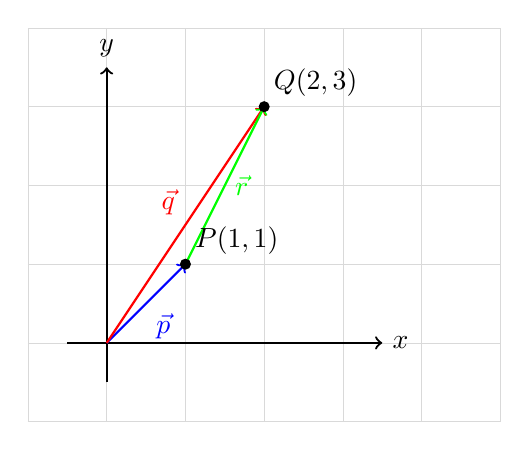
\begin{tikzpicture}
		% Draw grid
		\draw[help lines, color=gray!30] (-1,-1) grid (5,4);
		
		% Draw axes
		\draw[thick,->] (-0.5,0) -- (3.5,0) node[right] {$x$};
		\draw[thick,->] (0,-0.5) -- (0,3.5) node[above] {$y$};
		
		% Define points
		\coordinate (P) at (1,1);
		\coordinate (Q) at (2,3);
		
		% Draw vectors
		\draw[thick,->,blue] (0,0) -- (P) node[midway,below right] {$\vec{p}$};
		\draw[thick,->,red] (0,0) -- (Q) node[midway,above left] {$\vec{q}$};
		\draw[thick,->,green] (P) -- (Q) node[midway,right] {$\vec{r}$};
		% Draw and label points
		\fill (P) circle (2pt) node[above right] {$P (1,1)$};
		\fill (Q) circle (2pt) node[above right] {$Q (2,3)$};
		
	\end{tikzpicture}

	\begin{emphbox}
		$\overrightarrow{p} = \overrightarrow{OP} = \overrightarrow{P}$\\
		$\overrightarrow{q} = \overrightarrow{OQ} = \overrightarrow{Q}$\\
		$\overrightarrow{r} = \overrightarrow{PQ} = \overrightarrow{OQ} - \overrightarrow{OP} = \overrightarrow{q} - \overrightarrow{p}$\\
	\end{emphbox}
\end{sectionbox}
	
	